\documentclass[]{article}

\usepackage[italian]{babel}
\usepackage[margin=20mm, footskip = 20pt]{geometry}
\usepackage{array}
\usepackage{tabularx}
\usepackage{graphicx}
\usepackage{subfiles}
\usepackage{hyperref}
\usepackage{nameref}
\usepackage{titlesec}
\usepackage{longtable}
\usepackage[table]{xcolor}
\usepackage{titling}
\usepackage{lastpage}
\usepackage{ifthen}
\usepackage{calc}
\usepackage{soulutf8}
\usepackage{contour}
\usepackage{float}
\usepackage{fancyhdr}
\usepackage{multirow}
\usepackage{pgfgantt}
\usepackage{lscape}

\newcommand{\hr}{\par\vspace{-.1\ht\strutbox}\noindent\hrulefill\par}

\graphicspath{ {./}
	{./commons/res}
}

%--------------------------------------------------
% Comandi per inserire contenuto del documento
%--------------------------------------------------
\makeatletter

\newcommand\appendToGraphicsPath[1]{%
	\g@addto@macro\Ginput@path{{#1}}%
}

\newcommand{\setTitle}[1]{%
	\newcommand{\@phTitle}{#1}%
}
\newcommand{\phTitle}{\@phTitle}

\newcommand{\setDate}[1]{%
	\newcommand{\@phDate}{#1}%
}
\newcommand{\phDate}{\@phDate}

\newcommand{\setUso}[1]{%
	\newcommand{\@uso}{#1}%
}
\newcommand{\uso}{\@uso}

\newcommand{\setVersione}[1]{%
	\newcommand{\@versione}{#1}%
}
\newcommand{\versione}{\@versione}

\newcommand{\disabilitaVersione}{%
	\renewcommand{\setVersione}[1]{}%
	\renewcommand{\versione}{DISABILITATA}
}

\newcommand{\setResponsabile}[1]{%
	\newcommand{\@responsabile}{#1}%
}
\newcommand{\responsabile}{\@responsabile}

\newcommand{\setRedattori}[1]{%
	\newcommand{\@redattori}{#1}%
}
\newcommand{\redattori}{\@redattori}

\newcommand{\setVerificatori}[1]{%
	\newcommand{\@verificatori}{#1}%
}
\newcommand{\verificatori}{\@verificatori}

\newcommand{\setModifiche}[1]{%
	\newcommand{\@modifiche}{#1}%
}
\newcommand{\modifiche}{\@modifiche}

\makeatother 

%--------------------------------------------------
% Comandi per i documenti esterni e il glossario
%--------------------------------------------------

\newcommand{\dext}[1]{\textsc{#1\textsubscript{\textit{D}}}}

\newcommand{\glock}[1]{\textsc{#1\textsubscript{\textit{G}}}}

%--------------------------------------------------
% Comandi per impostare sottotitoli di quarto e quinto livello
%--------------------------------------------------

\setcounter{secnumdepth}{4}
\setcounter{tocdepth}{4}

\titleformat{\paragraph}
{\normalfont\normalsize\bfseries}{\theparagraph}{1em}{}
\titlespacing*{\paragraph}{0pt}{2.25ex plus 1ex minus .2ex}{1.5ex plus .2ex}

\titleformat{\subparagraph}
{\normalfont\normalsize\bfseries}{\thesubparagraph}{1em}{}
\titlespacing*{\subparagraph}{0pt}{1.75ex plus 1ex minus .2ex}{.75ex plus .1ex}

\appendToGraphicsPath{../../commons/res/}

%------------------------------
%
% COMANDI DI CONFIGURAZIONE
%
%------------------------------

\setTitle{Studio di Fattibilità}

\setVersione{1.0.0}

\setDate{03-01-2020}

\setResponsabile{Alessandro Chimetto}

\setRedattori{
    Matteo Alba\\&
	Giacomo Bulbarelli \\&
	Alessandro Chimetto \\&
	Alessandro Dindinelli\\&
    Lucia Fenu\\&
    Paolo Scanferlato\\&
	Valton Tahiraj
}

\setVerificatori{
	Giacomo Bulbarelli \\&
	Alessandro Chimetto \\&
	Alessandro Dindinelli\\&
	Valton Tahiraj
}

\setUso{Interno}

\setModifiche{
%%	Vers.	&	Nome					&	Ruolo		&	Data		&	Desrizione		  \\
    1.0.0   &   Alessandro Chimetto &   Responsabile&   03-01-2020  &   Approvazione Documento\\
	0.7.0	&	Alessandro Chimetto	&	Verificatore&	18-12-2020	&	Verificato studio C3\\
	0.7.0	&	Matteo Alba			&	Redattore	&	18-12-2020	&	Aggiunto studio C3\\
	0.6.0	&	Alessandro Chimetto		&	Verificatore&	17-12-2020	&	Verifica studio C4\\
    0.6.0   &   Paolo Scanferlato       &   Redattore   &   16-12-2020  &   Aggiunto studio C4\\
    0.5.0   &   Valton Tahiraj          &   Verificatore &  14-12-2020  &   Verifica studio C6\\
	0.5.0	&	Lucia Fenu	            &	Redattore	&	14-12-2020	&	Aggiunto studio C6\\
	0.4.0	&	Alessandro Chimetto		&	Verificatore&	14-12-2020	&	Verifica studio C5\\
	0.4.0   &   Giacomo Bulbarelli  	&   Redattore   &   14-12-2020  &   Aggiunto studio C5\\
	0.3.0	&	Giacomo Bulbarelli		&	Verificatore&	14-12-2020	&	Verifica studio C7\\
	0.3.0   &   Valton Tahiraj  		&   Redattore   &   14-12-2020  &   Aggiunto studio C7\\
	0.2.0	&	Valton Tahiraj			&	Verificatore&	14-12-2020	&	Verifica studio C2\\
	0.2.0	&	Alessandro Dindinelli	&	Redattore	&	13-12-2020	&	Aggiunto studio C2\\
	0.1.0	&	Alessandro Dindinelli	&	Verificatore&	13-12-2020	&	Verifica studio C1\\
	0.1.0	&	Alessandro Chimetto		&	Redattore	&	12-12-2020	&	Stesura iniziale + studio C1
}
\begin{document}

	% Direttive per la creazione del titolo tramite comando maketitle
\title{\huge \textsc{\phTitle{}} \\
	\vspace{11pt} \large \textsc{\phDate{}}}

\author{} % Non toccare
\date{} % Non toccare

%--------------------
% Frontespizio
%--------------------

% Logo del gruppo
\begin{figure}[t!]
	\centering
	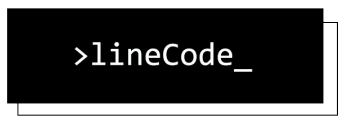
\includegraphics[width=20em]{lclong}
\end{figure}

% Titolo / Nome
\maketitle
\thispagestyle{empty}

% Dati specifici sul doc in forma tabulare
\begin{table}[ht]
	\begin{center}
		\label{tab:Dati sul documento}
		\begin{tabular}{r|l}
			\multicolumn{2}{c}{ \textsc{Dati sul documento} } \\
			\hline
			\textbf{Versione} & \versione{} \\
			\textbf{Uso} & \uso{}  \\
			\textbf{Redattori} & \redattori{} \\
			\textbf{Verificatori} & \verificatori{} \\
			\textbf{Responsabile} & \responsabile{} \\
			\textbf{Destinatari} & lineCode \\
								& prof.\ Vardanega Tullio \\		
								& prof.\ Cardin Riccardo \\
			\ifthenelse{\equal{\uso}{Esterno}}{
								& Sanmarco Informatica
			}{} \\
		\end{tabular}
	\end{center}
\end{table}

\newpage

\renewcommand{\arraystretch}{2} % allarga le righe con dello spazio sotto e sopra
\begin{longtable}[H]{>{\centering\bfseries}m{2cm} >{\centering}m{3.5cm} >{\centering}m{2.5cm} >{\centering}m{3cm} >{\centering\arraybackslash}m{5cm}}
	\rowcolor{lightgray}
	{\textbf{Versione}} & {\textbf{Nominativo}} & {\textbf{Ruolo}} & {\textbf{Data}} & {\textbf{Descrizione}}  \\
	\endfirsthead%
	\rowcolor{lightgray}
	{\textbf{Versione}} & {\textbf{Nominativo}}  & {\textbf{Ruolo}} & {\textbf{Data}} & {\textbf{Descrizione}}  \\
	\endhead%
	\modifiche{}%
\end{longtable}

	\newpage

	%--------------------------------
	%
	% IL CONTENUTO INIZIA DA QUI
	%
	%--------------------------------

	\tableofcontents
    \newpage

	\section{Introduzione}
		\subsection{Scopo del documento}
		Questo documento riporta lo studio svolto su ogni \glock{capitolato} proposto,
		enunciando per ognuno: finalità, tecnologie e caratteristiche ritenute
		negative o positive dai membri del gruppo.

		\subsection{Altri Documenti e Glossario}
		Terminologie specifiche all'interno del documento saranno scritte in \textsc{maiuscoletto} per evitare ambiguità e avranno a pedice:
		\begin{itemize}
			\item \textit{D} se indicano un documento specifico;
			\item \textit{G} se incluse nel \dext{glossario}.
		\end{itemize}

		\subsection{Riferimenti}
			\subsubsection{Normativi}
			\begin{itemize}
				\item \textbf{\dext{Norme di Progetto v1.0.0}}
			\end{itemize}

			\subsubsection{Informativi}
			\begin{itemize}
				\item \textbf{\glock{Capitolato} C1 - BlockCOVID: supporto digitale al contrasto della pandemia}\\
				(\url{https://www.math.unipd.it/~tullio/IS-1/2020/Progetto/C1.pdf});

				\item \textbf{\glock{Capitolato} C2 - EmporioLambda: piattaforma di e-commerce in stile Serverless}\\
				(\url{https://www.math.unipd.it/\~tullio/IS-1/2020/Progetto/C2.pdf});

				\item \textbf{\glock{Capitolato} C3 - GDP: Gathering Detection Platform}\\ (\url{https://www.math.unipd.it/~tullio/IS-1/2020/Progetto/C3.pdf});

				\item \textbf{\glock{Capitolato} C4 - HD Viz: visualizzazione di dati multidimensionali}\\
				(\url{https://www.math.unipd.it/~tullio/IS-1/2020/Progetto/C4.pdf});

				\item \textbf{\glock{Capitolato} C5 - PORTACS: piattaforma di controllo mobilità autonoma}\\
				(\url{https://www.math.unipd.it/~tullio/IS-1/2020/Progetto/C5.pdf});

				\item \textbf{\glock{Capitolato} C6 - RGP: Realtime Gaming Platform}\\
				(\url{https://drive.google.com/file/d/1MQ8j4plXMsKjBfLPrUfHCv\_6pfnjcU5T/view?usp=sharing});

				\item \textbf{\glock{Capitolato} C7 - SSD: soluzioni di sincronizzazione desktop}\\
				(\url{https://www.math.unipd.it/~tullio/IS-1/2020/Progetto/C7.pdf}).
			\end{itemize}

	\newpage

	\section{Valutazione capitolato scelto}
		\subsection{C5 - PORTACS}
			\subsubsection{Informazioni generali}
				\begin{itemize}
					\item \textbf{Titolo:} PORTACS;
					\item \textbf{Sottotitolo:} Piattaforma di controllo mobilità autonoma;
					\item \textbf{Proponente:} SanMarco Informatica;
					\item \textbf{Committente:} Prof. Tullio Vardanega e Prof. Riccardo Cardin.
				\end{itemize}

			\subsubsection{Descrizione}
			Il capitolato consiste nella creazione di un applicativo \glock{Real-Time} in grado di guidare delle unità dotate di mobilità autonoma in ambienti specifici, partendo dal presupposto che queste si muovano in ambienti in cui sono presenti altre unità (autonome o meno). In sede di presentazione sono stati riportati alcuni esempi di contesti in cui l'applicativo richiesto trova un senso di essere:
			\begin{itemize}
				\item automobili a guida autonoma;
				\item mezzi di per lo stock di merci all'interno di grandi magazzini, anch'essi dotati di guida autonoma;
				\item robot autonomi per il servizio al tavolo nel contesto della ristorazione.
			\end{itemize}

			\subsubsection{Finalità}
			Si vuole creare un applicativo che risulti diviso in:
			\begin{itemize}
				\item unità;
				\item sistema centrale.
			\end{itemize}
			Un'unità rappresenta un singolo mezzo dotato di mobilità autonoma che si muove nel contesto, definito da una serie di dati quali:
			 \begin{itemize}
			 	\item ID di sistema;
			 	\item velocità massima;
			 	\item posizione iniziale;
			 	\item lista ordinata dei \glock{POI} da visitare.
			 \end{itemize}

			Il Sistema-centrale si occupa di coordinare le singole unità, assicurandosi che ciascuna raggiunga la propria destinazione e che, nel farlo, non avvengano collisioni e siano rispettati dei vincoli imposti dall'ambiente in cui queste si muovono.
			Esso sarà definito tramite una mappatura dell'ambiente, potenzialmente partizionata in segmenti di dimensione fissa, e specificherà:
			\begin{itemize}
				\item percorrenze e relativi vincoli (sensi unici, numero massimo di unità contemporanee);
				\item definizione di \glock{POI}.
			\end{itemize}

			\subsubsection{Tecnologie}
			L'azienda non impone alcuna tecnologia specifica al gruppo da utilizzare in fase di sviluppo.
			In fase di consegna viene però richiesto l'impiego di:
			\begin{itemize}
				\item \textsc{\glock{Docker}}: software per la creazione di \glock{Container} istanziabili;
				\item \textsc{\glock{GitHub}}: piattaforma per lo sviluppo asincrono attraverso il tool di versionamento \glock{Git}.
			\end{itemize}

			\subsubsection{Linguaggi di programmazione}
			L'azienda non rende necessario l'uso di alcun linguaggio di programmazione al gruppo da utilizzare durante la fase di sviluppo.

			\subsubsection{Vincoli di progetto}
			Il progetto presenta dei vincoli sia per le singole unità, sia per il Sistema-centrale.

			\paragraph{Vincoli di progetto: Unità}
			Per quanto concerne le unità, queste dovranno essere caratterizzate da un insieme di elementi quali:
			\begin{itemize}
				\item punto di partenza nella griglia che rappresenta l'ambiente in cui l'unità si muove;
				\item velocità massima che l'unità può raggiungere;
				\item lista dei \glock{POI} che l'unità dovrà raggiungere.
			\end{itemize}

            \noindent
			Saranno poi dotate di una \glock{user-interface} così strutturata:
			\begin{itemize}
				\item indicatore della direzione dell'unità, rappresentante la direzione suggerita dal sistema centrale;
				\item indicatore della velocità corrente dell'unità, che non dovrà mai superare una soglia massima definita per ciascuna unità;
				\item pulsante per l'accensione/spegnimento dell'unità.
			\end{itemize}

			\paragraph{Vincoli di progetto: Sistema-centrale}
			Il sistema centrale presenterà una mappa dell'ambiente in cui le unità si muovono (considerando anche i vincoli dimensionali dello stesso) e sarà incaricato di indicare ad ognuna la prossima azione da intraprendere, in funzione di:
			\begin{itemize}
				\item prossimo \glock{POI} da raggiungere;
				\item posizione delle altre unità, consapevoli che:
					\begin{itemize}
						\item devono essere evitate collisioni;
						\item devono essere rispettati dei vincoli dimensionali definiti a priori;
						\item devono essere evitate collisione con agenti che non fanno parte dell'insieme delle unità (OPZIONALE).
					\end{itemize}
			\end{itemize}

            \noindent
			Sarà poi dotato anch'esso di una \glock{user-interface}, che permetterà di visualizzare:
			\begin{itemize}
				\item posizione \glock{real-time} delle singole unità;
				\item stato \glock{real-time} della mappa.
			\end{itemize}

			\subsubsection{Aspetti positivi}
			\begin{itemize}
				\item Il capitolato richiede l'utilizzo di \glock{Docker} tra le tecnologie obbligatorie, che risulta essere molto interessante per il gruppo;
				\item viene lasciata grande libertà rispetto alle tecnologie da impiegare in fase di sviluppo;
				\item in sede di presentazione è stata data molta importanza alla presentazione del problema da affrontare, che si è tradotta in una maggiore comprensibilità dello stesso;
				\item molti membri del gruppo apprezzano il tema affrontato.
			\end{itemize}
			\subsubsection{Criticità}
			\begin{itemize}
				\item Non tutti gli elementi del gruppo conoscono \glock{Docker};
				\item la grande libertà lasciata, se non gestita correttamente, potrebbe risultare un problema più che un vantaggio.
			\end{itemize}

			\subsubsection{Conclusioni}
				La scelta del gruppo è ricaduta su questo capitolato vista l'attualità dei temi trattati e alla luce di un'esposizione del problema chiara e convincente da parte dell'azienda proponente.
	\newpage

	\section{Valutazione capitolati non scelti}
		\subsection{C1 - BlockCOVID}
			\subsubsection{Informazioni generali}
			\begin{itemize}
				\item \textbf{Titolo:} BlockCOVID;
				\item \textbf{Sottotitolo:} Supporto digitale al contrasto della pandemia;
				\item \textbf{Proponente:} Imola Informatica;
				\item \textbf{Committente:} Prof. Tullio Vardanega e Prof. Riccardo Cardin.
			\end{itemize}

			\subsubsection{Descrizione}
			Vista la corrente pandemia di SARS-CoV-2 e conseguenti accordi fra sindacati e imprese, si vuole creare un'applicazione in grado di tracciare la presenza del personale di un organizzazione (es. scuola o azienda) nelle proprie postazioni di lavoro e di tracciare l'igienizzazione di quest'ultime da parte dell'utente o un'azienda specializzata.

			\subsubsection{Finalità}
			Si vuole creare un'applicazione mobile che permetta all'utente di:
			\begin{itemize}
				\item segnalare, tramite tag \glock{RFID}, l'occupazione di una postazione di lavoro ad un server dedicato;
				\item prenotare una postazione libera ed igienizzata;
				\item segnalare se la postazione è stata pulita autonomamente alla fine dell'utilizzo.
			\end{itemize}
			L'azienda esterna specializzata deve poter utilizzare l'applicazione per:
			\begin{itemize}
				\item ricevere una lista delle postazioni da igienizzare;
				\item marcare la stanza come igienizzata.
			\end{itemize}
			Il server dedicato deve tenere traccia delle informazioni in una struttura dati di tipo \glock{blockchain} e deve mettere a disposizione dell'amministratore:
			\begin{itemize}
				\item un'interfaccia che consenta di creare, modificare o eliminare postazioni e stanze;
				\item la gestione del calendario delle prenotazioni;
				\item la possibilità di eseguire ricerche e creare report su personale addetto e igienizzazioni.
			\end{itemize}

			\subsubsection{Tecnologie}
			Parte dell'interesse di ricerca dell'azienda è l'esplorazione di nuove soluzioni tecnologiche dunque quasi tutte le tecnologie da essa proposte non sono obbligatorie ma solamente consigliate sulla base dell'esperienza:
			\begin{itemize}
				\item \textsc{\glock{API Rest} o \glock{gRPC}:} tecnologie di comunicazione asincrona fra applicazione e server;
				\item \textsc{\glock{Ethereum}:} tecnologia \glock{blockchain} per immagazzinare dati con opponibilità a terzi;
				\item \textsc{\glock{Kubernetes}, \glock{Openshift} o \glock{Rancher}:} orchestratori per gestire \glock{deploy} e scalabilità delle componenti server.
			\end{itemize}

			\subsubsection{Linguaggi di Programmazione}
			\begin{itemize}
				\item \textsc{\glock{Java}, \glock{Python} o \glock{Node.js}:} linguaggi molto diffusi, consigliati (ma non obbligatori) per lo sviluppo delle componenti \glock{back-end};
				\item \textsc{\glock{Kotlin} o \glock{Swift}:} linguaggi per lo sviluppo di applicazioni mobile rispettivamente su piattaforme \glock{Android} e \glock{iOS};
				\item \textsc{\glock{Solidity} o \glock{Vyper}:} linguaggi per lo sviluppo di \glock{smart contract} per la piattaforma \glock{Ethereum}.
			\end{itemize}

			\subsubsection{Vincoli di Progetto}
			\begin{itemize}
				\item Per la comunicazione asincrona fra applicazione e server, si richiede di utilizzare \glock{API Rest} o in alternativa \glock{gRPC};
				\item scansione dei codici nel tempo sufficiente a certificare la presenza della persona in postazione;
				\item presentazione di un resoconto su scelte e test effettuati per garantire una buona durata della batteria del dispositivo mobile nonostante l'utilizzo del lettore \glock{RFID};
			\end{itemize}

			\subsubsection{Aspetti positivi}
			\begin{itemize}
				\item Si sta affrontando un tema di grande attualità e la sua realizzazione, potenzialmente, implicherebbe un contributo anche a livello sociale;
				\item il \glock{capitolato} è fortemente politematico in quanto spazia dall'uso di hardware specializzato all'uso di linguaggi di programmazione attuali e strumenti rilevanti nell'ambito \glock{DevOps} per non parlare dell'utilizzo della struttura dati \glock{blockchain}; tutto ciò rende il lavoro proposto molto stimolante.
			\end{itemize}

			\subsubsection{Criticità}
			\begin{itemize}
				\item Il fatto che questo \glock{capitolato} sia estremamente politematico implica che la mole di lavoro nel progetto da esso derivato sia imponente. Ci sono molte tecnologie nuove da imparare in poco tempo e al fine di soddisfare i soli requisiti obbligatori si richiede lo sviluppo di due applicazioni di più che modeste dimensioni (mobile e server) che implementino tutte le tecnologie;
				\item non è chiaro se l'hardware specifico per tag \glock{RFID} venga fornito dall'azienda e in che quantità; ciò potrebbe diventare un problema nel momento in cui le unità a disposizione fossero poche in quanto poche persone ne avrebbero accesso e, vista la mancanza di contatti causa pandemia, non ci sarebbe la possibilità di scambiarle con altri membri del gruppo.
			\end{itemize}

			\subsubsection{Conclusioni}
			Nonostante il questo \glock{capitolato} abbia suscitato un forte interesse in tutti i membri del gruppo per questioni sia tecnologiche che sociali, si teme che la mole di lavoro sia troppo ampia e di conseguenza che non si riesca a consegnare il prodotto in tempi accettabili per il gruppo.

		\newpage

		\subsection{C2 - Emporio Lambda}

		\subsubsection{Informazioni generali}
			\begin{itemize}
				\item \textbf{Titolo:} Emporio Lambda;
				\item \textbf{Proponente:} Red Babel;
				\item \textbf{Committente:} Prof. Tullio Vardanega e Prof. Riccardo Cardin.
			\end{itemize}

			\subsubsection{Descrizione}
			Le piattaforme di \glock{e-commerce} possono essere triviali, come pure complesse, in base alle funzionalità che si vogliono garantire. Inoltre i bisogni delle aziende possono variare ampiamente nel tempo e si scopre quindi la necessità di appoggiarsi a tecnologie affidabili per l'uso richiesto, e che garantiscano adattabilità a cambiamenti futuri.

			\subsubsection{Finalità}
			Emporio Lambda mira ad essere una piattaforma di \glock{e-commerce} con architettura \glock{serverless} appoggiandosi ad \glock{AWS}. Si vogliono garantire le funzionalità tipiche di una piattaforma commerciale, che permetta agli amministratori un'adeguata gestione degli ordini e dell'inventario, ed agli utenti un'ottima esperienza di ricerca ed acquisto dei prodotti disponibili.
			\\
			Il sito dovrà essere performante e garantire agli utenti un accesso immediato alla ricerca dei prodotti. Sarà importante l'uso di tecniche di \glock{SEO} soprattutto per le pagine dei prodotti in vendita.
			\\
			Dovrà essere disponibile uno strumento di autenticazione, che potrà essere realizzato appoggiandosi ad \glock{Amazon Cognito}.

			\subsubsection{Tecnologie}
			\begin{itemize}
				\item \textsc{\glock{AWS Lambda}:} piattaforma di calcolo serverless, fornita come parte di \glock{AWS} che si occupa della gestione \glock{back-end} di applicazioni web;
				\item \textsc{\glock{Amazon CloudWatch}:} servizio di monitoraggio e osservabilità che raccoglie dati di monitoraggio e operativi sotto forma di log, parametri ed eventi, fornendo una visualizzazione unificata delle risorse;
				\item \textsc{\glock{Amazon Cognito}:} servizio la gestione di registrazione e controllo degli accessi a piattaforme web.
			\end{itemize}

			\subsubsection{Linguaggi di Programmazione}
			\begin{itemize}
				\item \glock{Next.js}: framework per lo sviluppo \glock{front-end} di siti web;
				\item \glock{Typescript}: linguaggio che va ad estendere \glock{Javascript} dotandolo di tipizzazione;
				\item \glock{Node.js}: linguaggio molto diffuso, per lo sviluppo delle componenti \glock{back-end} da appoggiare ad \glock{AWS}.
			\end{itemize}


			\subsubsection{Vincoli di Progetto}
			Il sito deve permettere il supporto ai ruoli di:
			\begin{itemize}
			    \item amministratore di sistema: per la configurazione ed amministrazione del sito;
			    \item venditore: per l'organizzazione e la gestione dei prodotti e delle loro informazioni;
			    \item cliente: utente generico del sito che può visualizzare ed acquistare i prodotti.
			\end{itemize}
		A livello di funzionalità per il cliente, devono essere previste le seguenti pagine:
        \begin{itemize}
            \item homepage;
            \item profilo utente;
            \item elenco prodotti;
            \item dettagli prodotti;
            \item carrello;
            \item checkout.
        \end{itemize}
		Si deve poi garantire un'adeguata integrazione con i servizi amministrativi tipici di questo ambiente, come:
        \begin{itemize}
            \item supporto utenti;
            \item tracciamento delle operazioni;
            \item inventario magazzino.
        \end{itemize}

			\subsubsection{Aspetti positivi}
			\begin{itemize}
				\item Le tecnologie richieste per la realizzazione del \glock{capitolato} sono state giudicate di interesse;
				\item la difficoltà generale dei requisiti è considerata adeguata per i componenti del gruppo.
			\end{itemize}

			\subsubsection{Criticità}
			\begin{itemize}
			    \item L'\glock{e-commerce} è stato considerato come un target non stimolante da parte del gruppo;
				\item il materiale reso disponibile dal proponente è stato giudicato non molto chiaro, e si ha il timore che ci potrebbero essere problemi di cooperazione in futuro.
			\end{itemize}

			\subsubsection{Conclusioni}
			Nonostante le tecnologie che si andrebbero ad usare sembrino interessanti, nel complesso il \glock{capitolato} non ha suscitato interesse sufficiente rispetto alle altre opzioni disponibili al gruppo.

		\newpage

		\subsection{C3 - GDP}
		\subsubsection{Informazioni generali}
		\begin{itemize}
			\item \textbf{Titolo:} GDP;
			\item \textbf{Sottotitolo:} Gathering Detection Platform;
			\item \textbf{Proponente:} Sync Lab;
			\item \textbf{Committente:} Prof. Tullio Vardanega e Prof. Riccardo Cardin.
		\end{itemize}

		\subsubsection{Descrizione}
		In seguito alla pandemia del virus COVID-19 scoppiata negli ultimi mesi sono sorti numerosi problemi. Dopo un periodo di quarantena forzata la vita doveva ripartire ed ai cittadini è stata permessa la circolazione. Durante la vita quotidiana si generano spesso assembramenti in numerosi luoghi e per non aggravare la situazione bisogna cercare di prevenire questo problema. Grazie all’informatica possiamo quindi scongiurare l’aggravarsi della situazione dovuta ai problemi sociali legati all’affollamento.

		\subsubsection{Finalità}
		Si vuole creare un’applicazione web che permetta di:
		\begin{itemize}
		\item misurare tramite dei contapersone e date le immagini/video delle videocamere di contare le persone a bordo dei mezzi pubblici;
		\item poter acquisire continuativamente nel tempo e in modalità a bassa latenza delle informazioni raccolte da dispositivi di flussi dati;
		\item elaborare in tempo reale i dati acquisiti per rappresentare le variazioni nel tempo dei dati monitorati, come ad esempio la variazione dei flussi delle persone in ambienti urbani; confrontare e correlare tra loro dati provenienti da flussi diversi, ad esempio correlando i dati raccolti a bordo dei mezzi di trasporto di interesse con i dati raccolti in prossimità delle aree di interesse quali ad esempio fermate di autobus, strade dedicate al traffico veicolare, zone urbane; è poi fondamentale archiviare tutti i dati acquisiti ed i risultati delle loro elaborazioni affinché siano conservati nel tempo e comunque disponibili in qualunque caso sia richiesto il loro utilizzo;
		\item identificazione, a partire dai dati acquisiti ed elaborati, di eventi che nel tempo sono risultati aver concorso ad esempio all’insorgere di alterazioni significative del flusso di utenti;
		\item previsione dell’insorgenza futura di variazioni significative di flussi di persone al fine di poter fornire degli indicatori automatici in grado di fornire supporto alle decisioni da parte del personale tecnico specializzato preposto a tale scopo.
		\end{itemize}

		\subsubsection{Tecnologie}
		Ci sono alcune scelte preferenziali per lo svolgimento del progetto:
		\begin{itemize}
		\item utilizzo di \glock{Java} e \glock{Angular} per lo sviluppo delle parti di \glock{Back-end} e \glock{Front-end} della componente Application del sistema;
		\item il framework \glock{Leaflet} per la gestione delle mappe \glock{heatmap};
		\item utilizzo di protocolli asincroni per le comunicazioni tra diverse componenti;
		\item utilizzo del pattern \glock{Publisher/Subscriber} e adozione del protocollo \glock{MQTT}(‘MQ Telemetry Transport or Message Queue Telemetry Transport’).
		\end{itemize}

		\subsubsection{Aspetti positivi}
		Il progetto risultava secondo il gruppo uno dei tre capitolati più interessanti e stimolanti:
		\begin{itemize}
		\item il problema da affrontare è qualcosa che riguarda la vita di tutti i giorni e che potrebbe portare a miglioramenti anche fuori da una situazione di emergenza COVID-19;
		\item le tecnologie richieste per risolvere il problema e la componente di \glock{IA} rappresenta un’ottima occasione per ampliare il bagaglio di conoscenze.
		\end{itemize}

		\subsubsection{Criticità}
		\begin{itemize}
		\item La parte di \glock{IA} e la problematica da risolvere sembrava meno interessante rispetto al capitolato scelto.
		\end{itemize}

		\subsubsection{Conclusioni}
		Dopo aver preso ampiamente in considerazione il capitolato in questione ed aver seguito la presentazione ed il seminario tecnologico il gruppo ha preferito orientarsi verso un’altra scelta che sembrava più stimolante.

		\newpage

		\subsection{C4 - HD Viz}
		\subsubsection{Informazioni generali}
		\begin{itemize}
			\item \textbf{Titolo:} HD Viz;
			\item \textbf{Sottotitolo:} Visualizzazione di dati multidimensionali;
			\item \textbf{Proponente:} Zucchetti;
			\item \textbf{Committente:} Prof. Tullio Vardanega e Prof. Riccardo Cardin.
		\end{itemize}

		\subsubsection{Descrizione}
		Nella gestione di grandi volumi di dati si distinguono quattro fasi fondamentali:
		\begin{itemize}
			\item acquisizione;
			\item pulizia;
			\item analisi;
			\item interpretazione.
		\end{itemize}
		L'ultima, l'interpretazione, si suddivide in due ulteriori fasi: la prima esplorazione, chiamata \glock{Exploratory Data Analysis} (EDA), e la modellazione dei fenomeni rilevati.
		Il capitolato in questione prende in considerazione proprio l'esplorazione tramite la visualizzazione grafica del dato in molte dimensioni.

		\subsubsection{Finalità}
		Si vuole quindi creare un'applicazione di visualizzazione grafica di dati con molte dimensioni a supporto della fase esplorativa dell’analisi dei dati.
		Il software dovrà poter visualizzare i dati in almeno 15 dimensioni e utilizzando questi metodi:
		\begin{itemize}
			\item \glock{Scatter plot Matrix} (fino ad un massimo di 5 dimensioni);
			\item \glock{Force Field};
			\item \glock{Heat Map};
			\item \glock{Proiezione Lineare Multi Asse}.
		\end{itemize}

		\subsubsection{Tecnologie e Linguaggi di Programmazione}
		L’applicazione “HD Viz” di visualizzazione dei dati a molte dimensioni dovrà essere sviluppata prevalentemente in tecnologia \glock{HTML}/\glock{CSS}/\glock{JavaScript} utilizzando la libreria \glock{D3.js}.
		La parte server di supporto alla presentazione nel \glock{browser} e alle \glock{query} ad un database \glock{SQL} o \glock{NoSQL} potrà essere sviluppata in \glock{Java} con server \glock{Tomcat} o in \glock{Javascript} con server \glock{Node.js}.
		Per lo sviluppo di algoritmi di preparazione del dato per la visualizzazione (requisito opzionale del capitolato), l'azienda mette a disposizione alcune librerie per gli algoritmi:
		\begin{itemize}
			\item \glock{t-SNE};
			\item \glock{UMAP};
			\item \glock{Self Organizing Map};
			\item \glock{Learning Vector Quantization}.
		\end{itemize}

		\subsubsection{Vincoli di Progetto}
		Il capitolato prevede dei requisiti obbligatori e opzionali:
		\begin{itemize}
			\item i dati da prendere in esame dovranno poter avere almeno fino a 15 dimensioni, ma deve essere possibile visualizzarne anche con meno;
			\item il sistema di visualizzazione accetterà i dati da un file in formato \glock{CSV} o da una \glock{query} ad un database;
			\item devono essere implementate almeno 4 metodologie di visualizzazione: \glock{Scatter Plot Matrix} (max 5 dimensioni), \glock{Force Field}, \glock{Heat Map}, \glock{Proiezione lineare Multi Asse};
			\item nel grafico \glock{Heat Map} i punti dovranno essere ordinati;
			\item sviluppare altri metodi di visualizzazione con più di tre dimensioni (opzionale);
			\item utilizzare funzioni di calcolo della distanza diverse dalla distanza “Euclidea” in tutte le visualizzazioni che dipendono da tale concetto (opzionale);
			\item utilizzare funzioni di “forza” diverse da quelle previste in automatico dal grafico \glock{force based} di \glock{D3} (opzionale);
			\item implementare analisi automatiche per evidenziare situazioni di particolare interesse. Esempi di questa possibilità si possono vedere in \glock{ggobi} e \glock{Orange Canvas} (opzionale);
			\item sviluppare algoritmi di preparazione del dato per la visualizzazione, cioè anziché eseguire la trasformazione direttamente nella visualizzazione far precedere un passo di trasformazione (opzionale).
		\end{itemize}
		Inoltre, l'azienda fa sapere che valuterà altre proposte e se verranno ritenute valide saranno considerate come requisito opzionale.

		\subsubsection{Aspetti positivi}
		Da qualche anno ormai i \glock{Big Data} sono una componente fondamentale di molte aziende e probabilmente con il passare del tempo il fenomeno aumenterà. L'analisi di questi dati è quindi importantissima e di stretta attualità e la possibilità di imparare a sfruttare le tecnologie utilizzate in questo campo rende il capitolato molto interessante. Inoltre permetterebbe il richiamo ad alcune affascinanti discipline studiate negli anni passati come le basi di dati, la statistica e ovviamente la programmazione.

		\subsubsection{Criticità}
		Contesto troppo monotematico. Buona parte dello sviluppo in \glock{javascript}.

		\subsubsection{Conclusioni}
		Si teme che una buona parte del lavoro sia monotematica visto che sarà realizzata con un ristretto insieme di tecnologie e quindi ritenuta poco stimolante dalla maggioranza del gruppo.

		\newpage


        \subsection{C6 - Realtime Gaming Platform }
		\subsubsection{Informazioni generali}
		\begin{itemize}
			\item \textbf{Titolo:} Realtime Gaming Platform;
			\item \textbf{Proponente:} Zero12;
			\item \textbf{Committente:} Prof. Tullio Vardanega e Prof. Riccardo Cardin.
		\end{itemize}

		\subsubsection{Descrizione}
		Sviluppo e progettazione di un videogioco a scorrimento verticale fruibili su dispositivi mobile con la possibilità di giocare anche in \glock{multiplayer} oltre alla campagna in \glock{singleplayer}.

		\subsubsection{Finalità}
		Il fulcro è la progettazione di un sistema \glock{multiplayer} “fantasma” in cui i giocatori non possano interagire tra loro, ma solo controllare in \glock{real-time} le mosse dell'avversario senza poter intervenire.
		La modalità \glock{singleplayer} sarà di tipo infinito, con difficoltà crescente, fino a che il giocatore non avrà esaurito le vite o i \glock{power-up} in suo possesso.
		Al termine della progettazione, dovranno essere forniti i seguenti materiali:
		\begin{itemize}
			\item report/retrospettiva sulle tecnologie utilizzate per capire se la scelta iniziale è stata corretta;
			\item configurazione dell'architettura \glock{cloud} ed eventualmente il codice sorgente tramite \glock{git} (se il servizio lo prevede);
			\item codice sorgente dell'applicazione tramite \glock{repository} \glock{git}.
		\end{itemize}

		\subsubsection{Tecnologie}
		Le tecnologie consigliate dall'azienda riguardano principalmente \glock{AWS}, che fornisce servizi di \glock{cloud} computing; dando libertà di scelta sull'uso dei servizi offerti da tale tecnologia, motivandone poi la scelta.
		Su consiglio:
		\begin{itemize}
			\item \glock{AWS Gamelift}: servizio specializzato in giochi \glock{multiplayer};
			\item \glock{AWS Appsync}: tecnologia che permette l'utilizzo del linguaggio \glock{GraphQL} in modo semplice e sicuro.

		\end{itemize}

		\subsubsection{Linguaggi di Programmazione}
		\begin{itemize}
			\item \glock{Node.js}: linguaggio per lo sviluppo delle componenti \glock{back-end};
			\item \glock{Kotlin}: linguaggio per lo sviluppo di applicazioni mobile per piattaforme \glock{Android} (richiesta minima Android 8);
			\item \glock{Swift}: linguaggio per lo sviluppo di applicazioni mobile per piattaforme \glock{iOS}(richiesta minima iOS 13);
			\item \glock{GraphQL}: linguaggio di manipolazione e \glock{query} di dati \glock{Open Source} per \glock{API} e un runtime per la realizzazione di \glock{query} con dati esistenti.
		\end{itemize}

		\subsubsection{Vincoli di Progetto}
		\begin{itemize}
			\item Svolgere un'analisi preliminare sulle tecnologie \glock{AWS}, motivandone la scelta;
			\item l'architettura server dovrà essere scalabile, che sarà una delle caratteristiche che influenzeranno la scelta dell'\glock{AWS}.
		\end{itemize}

		\subsubsection{Aspetti positivi}
		\begin{itemize}
			\item La libertà che l'azienda offre sulla scelta delle tecnologie da utilizzare;
			\item la disponibilità nello studio preliminare dei diversi servizi \glock{cloud};
			\item \glock{repository} \glock{git} offerta dalla azienda per lo sviluppo del progetto.
		\end{itemize}

		\subsubsection{Criticità}
		\begin{itemize}
			\item Non avendo esperienza sulle tecnologie offerte non è chiara la mole di lavoro che si affronterà, in particolare sullo studio individuale;
			\item troppa libertà di scelta potrebbe essere difficile da gestire se non si hanno le competenze preliminari e quindi richiederebbe lavoro aggiuntivo per la conoscenza di un numero abbastanza sufficiente per la scelta finale da utilizzare al fine di un ragionato sviluppo nell'ambiente di lavoro.
		\end{itemize}

		\subsubsection{Conclusioni}
		Per quanto l'argomento videogiochi sia sempre ben gradito all'interno del gruppo, il team non ha le conoscenze adatte per soddisfare i requisiti nei tempi stabiliti, in particolare per la libera scelta che il proponente offre.
		Riteniamo comunque che sia una buona proposta, ma non per le nostre competenze generali attuali difficilmente sanabili in tempo utile.

		\newpage

        \subsection{C7 - SSD}
            \subsubsection{Informazioni generali}
            \begin{itemize}
                \item \textbf{Titolo:} SSD;
                \item \textbf{Sottotitolo:} soluzioni di sincronizzazione desktop;
                \item \textbf{Proponente:} ZEXTRAS;
                \item \textbf{Committente:} Prof. Tullio Vardanega e Prof. Riccardo Cardin.
            \end{itemize}

            \subsubsection{Descrizione}
            Si vuole approfondire il mondo degli algoritmi di sincronizzazione desktop, essendo la piattaforma principale per molti utenti professionali, in un modo non triviale che non si limiti a permettere il lavoro in un dispositivo mantenendo una copia del lavoro salvata su \glock{Cloud}.

            \subsubsection{Finalità}
            I principali obiettivi di questo progetto sono:
            \begin{itemize}
                \item sviluppo di un algoritmo solido ed efficiente in grado di garantire il salvataggio in \glock{Cloud} del lavoro e contemporaneamente la sincronizzazione dei cambiamenti presenti in \glock{Cloud};
                \item sviluppo di un'interfaccia multipiattaforma per l'uso dell'algoritmo nei più importanti sistemi operativi desktop esistenti(\glock{MacOs}, \glock{Windows}, \glock{Linux});
                \item utilizzo dell'algoritmo sviluppato per richiedere e fornire i cambiamenti ai contenuti in sincronizzazione verso il prodotto del proponente \glock{Zextras Drive}.
            \end{itemize}
            Le principali funzioni richieste sono:
            \begin{itemize}
                \item configurazione ed autenticazione dell'utente;
                \item gestione di cosa sincronizzare e di cosa ignorare nelle cartelle \glock{Cloud};
                \item gestione di cosa sincronizzare e di cosa ignorare nelle cartelle locali;
                \item sincronizzazione costante dei cambiamenti, siano essi locali o remoti;
                \item possibilità di modifica delle preferenze a posteriori;
                \item sistema di notifica utente dei cambiamenti.
            \end{itemize}
            Con l'aggiunta di funzionalità avanzate quali:
            \begin{itemize}
                \item gestione delle condivisioni;
                \item integrazione protocollo \glock{MAPI}.
            \end{itemize}

            \subsubsection{Tecnologie}
            Il proponente sancisce che la soluzione sviluppata non dipenda da installazione di \glock{Framework} terzi per funzionare.
            Consiglia quindi l'uso dei seguenti \glock{Framework}:
            \begin{itemize}
                \item \glock{Qt Framework}: \glock{Framework} consigliato per lo sviluppo dell'interfaccia e del controller d'architettura;
                \item \glock{Python}: linguaggio consigliato per lo sviluppo della Backend Business Logic.
            \end{itemize}


            \subsubsection{Aspetti positivi}
            \begin{itemize}
                \item Le tecnologie sono conosciute dalla maggior parte dei membri del gruppo.
            \end{itemize}

            \subsubsection{Criticità}
            \begin{itemize}
                \item La documentazione del \glock{capitolato} risulta scritta in modo approssimato facendo perdere al gruppo l'entusiasmo di lavorare con questo proponente;
                \item l'idea risulta poco innovativa.
            \end{itemize}

            \subsubsection{Conclusioni}
            Questo \glock{capitolato} non ha suscitato interesse in nessun membro del gruppo. Il gruppo ha quindi deciso di concentrarsi su altri \glock{capitolati}.
\end{document}

